\subsection{Uplifted}
\label{sec:specie-uplifted}

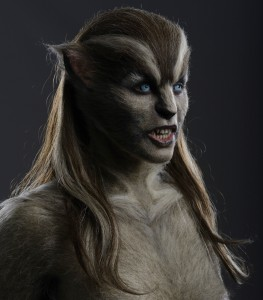
\includegraphics[width=\linewidth]{wolves-movie-still-1-263x300}

Uplifted is the general name given to the genetically-engineered animals that have been given basic sentience and humanoid features. The original reason behind this science experiment has long been lost, but many tech-heads speculate that the Uplifted were supposed to perform the menial labour on planets that could not support a Bot network. Regardless, the Uplifted are still treated as an inferior species because of their artificial evolution.

Uplifted physically range wildly across the spectrum from humanoid to their base animal form, but all Uplifted have at least a humanoid-style torso that have two arms with opposable thumbs (for manipulating objects). Faces may or may not have a prominent snout, and some uplifted do not have a tail. Almost all Uplifted have the fur coat of their base animal base form, but some choose to partially shave or style it to better fit in humanoid society.

Due to their severe genetic alteration and base animal genetics, Uplifted cannot breed with humans or with their animal precedessors. This does not deter kinky humanoids, and many unsavoury places in the Black offer "special" Uplifted services. However the heart wants what it wants, and Uplifted-Human couples are a rare sight in the Black. These couples generally seek out geneticists who are able to splice their DNA into viable offspring.

To create an Uplifted character, please refer to the \textit{\hyperref[sec:rules-creation]{Character creation section}}
